\documentclass[a4paper]{article}
\usepackage[utf8]{inputenc}
\usepackage{amsmath}
\usepackage{amssymb}
\usepackage{mathtools}
\usepackage{amsfonts}
\usepackage{lastpage}
\usepackage{tikz}
\usepackage{float}
\usepackage{textcomp}
\usetikzlibrary{patterns}
\usepackage{pdfpages}
\usepackage{gauss}
\usepackage{fancyvrb}
\usepackage[table]{colortbl}
\usepackage{fancyhdr}
\usepackage{graphicx}
\usepackage[margin=2.5 cm]{geometry}

\definecolor{listinggray}{gray}{0.9}
\usepackage{listings}
\lstset{
	language=,
	literate=
		{æ}{{\ae}}1
		{ø}{{\o}}1
		{å}{{\aa}}1
		{Æ}{{\AE}}1
		{Ø}{{\O}}1
		{Å}{{\AA}}1,
	backgroundcolor=\color{listinggray},
	tabsize=3,
	rulecolor=,
	basicstyle=\scriptsize,
	upquote=true,
	aboveskip={0.2\baselineskip},
	columns=fixed,
	showstringspaces=false,
	extendedchars=true,
	breaklines=true,
	prebreak =\raisebox{0ex}[0ex][0ex]{\ensuremath{\hookleftarrow}},
	frame=single,
	showtabs=false,
	showspaces=false,
	showlines=true,
	showstringspaces=false,
	identifierstyle=\ttfamily,
	keywordstyle=\color[rgb]{0,0,1},
	commentstyle=\color[rgb]{0.133,0.545,0.133},
	stringstyle=\color[rgb]{0.627,0.126,0.941},
  moredelim=**[is][\color{blue}]{@}{@},
}

\lstdefinestyle{base}{
  emptylines=1,
  breaklines=true,
  basicstyle=\ttfamily\color{black},
}

\pagestyle{fancy}
\def\checkmark{\tikz\fill[scale=0.4](0,.35) -- (.25,0) -- (1,.7) -- (.25,.15) -- cycle;} 
\newcommand*\circled[1]{\tikz[baseline=(char.base)]{
            \node[shape=circle,draw,inner sep=2pt] (char) {#1};}}
\newcommand*\squared[1]{%
  \tikz[baseline=(R.base)]\node[draw,rectangle,inner sep=0.5pt](R) {#1};\!}
\cfoot{Page \thepage\ of \pageref{LastPage}}
\DeclareGraphicsExtensions{.pdf,.png,.jpg}
\author{Nikolaj Dybdahl Rathcke (rfq695)}
\title{Fifth Home Assignment \\ Data Analysis}
\lhead{Nikolaj Dybdahl Rathcke (rfq695)}
\chead{Data Analysis}
\rhead{Assignment 5}

\begin{document}
\maketitle
\section*{Question 1}
\subsection*{(1)}
The VC-dimension is $3$. No matter how you label the points that makes an equilateral triangle, it can be shattered. However, if you have four points, the diagonal can be the same length, in which case if you label the points in one diagonal one thing, and the other something else, they cannot be shattered. If one diagonal is larger than the other, then if these two points in that diagonal are labeled positive, it cannot be shattered, thus $d_{VC}(\mathcal{H})=3$.


\subsection*{(2)}
The VC-dimension is $\infty$. Consider placing $n$ points in a circle. If it is all the convex sets, we can always connect $2$ points without including any other point. It does not matter what $n$ is, so $d_{VC}(\mathcal{H})=\infty $.


\subsection*{(3)}
Consider points in a circle where the points make a polygon. With all convex sets, the equation (2.14) makes a very loose bound since $d_{VC}=\infty$, while it for circles in $\mathbb{R}^2$ is tighter as $d_{VC}=3$.

\subsection*{(4)}
The VC-dimension is $2$. This case is very easy as you simply put the $2$ point next to each other, and they can be shattered. However, with $3$ points, we have to place them within $180$ degrees of the origin as it cannot be shattered if all points are labeled the same otherwise. This means we place $3$ points with some degree from the origin. If the point in middle (another point lies at a degree $x$ which is more than that and another point lies at a degree $y$ which is less than that) is labeled differently than the two other points, it cannot be shattered. Therefore, $d_{VC}(\mathcal{H})=2$.


\subsection*{(5)}
The VC-dimension is $3$. Three points that lie in a triangle, no matter what label, can be shattered. But when there are four points, if the points on a diagonal are labeled the same, but differently than the two others on the other diagonal, it cannot be shattered.

\subsection*{(6)}
To determine this, we use equation (2.14) in [LFD] that says
\begin{align*}
E_{out}(g)&\leq E_{in}(g)+\sqrt{\frac{8}{N}\ln(\frac{4((2N)^{d_{VC}}+1)}{\delta}} \\
\Leftrightarrow E_{out}(g)-E_{in}(g)&\leq \sqrt{\frac{8}{N}\ln(\frac{4((2N)^{d_{VC}}+1)}{\delta}} 
\end{align*}
So we need to solve for $N$ on the right side, so it is $0.05$ with $\delta=0.05$ and $d_{VC}=10$.\\
This gives the answer $N=452957$ which is the sample size needed.

\newpage
\section*{Question 2}
We have the following
\begin{align*}
X=
\begin{bmatrix}
0 & 0 \\
0 & -1 \\
-2 & 0
\end{bmatrix}
\ \ \ \
y=
\begin{bmatrix}
-1 \\
-1 \\
1
\end{bmatrix}
\end{align*}
We get the inequalities
\begin{align*}
-b&\geq 1 &(i) \\  
w_2-b&\geq 1 &(ii) \\
-2w_1+b&\geq 1 &(iii)
\end{align*}
Combining (i) and (ii) gives
\begin{align*}
w_2\geq 0 \\ 
\end{align*}
And combining (i) and (iii) gives
\begin{align*}
w_1\leq -1 \\ 
\end{align*}
This means the following
\begin{align*}
(b^*=-1,w_1^*=-1,w_2^*=0)
\end{align*}
makes the optimal hyperplane. It has the margin
\begin{align*}
\frac{1}{\|w^*\|}=\frac{1}{\sqrt{1}}=1
\end{align*}

\newpage
\section*{Question 3}
\subsection*{(1)}
One way to generate random points is to first pick an angle in $[0, 2\pi)$, then pick a random length in $[0,1]$ and then find the corresponding $x$ and $y$-coordinates. Let $\theta$ be the angle and let $c$ be the length, then the coordinates $(x,y)$ are given by
\begin{align*}
x&=\frac{c\cdot sin(\theta)}{\sin(\pi/2)} \\
y&=\sqrt{c^2-x^2}
\end{align*}
Using the law of sines to find $x$ and then using the Pythagorean theorem to find $y$.

\newpage
\section*{Question 4}
We want to implement and apply a soft-margin SVM to the MNINST dataset. The soft SVM solution which was uploaded to absalon has been used.\\
First we build a classifier for distinguishing between digits "0" and "1", which we test with the first 250, 500, and 1000 occurences of the digits from the training set. Then we apply soft-margin SVM with $C= [10^{-6},10^{-5},10^{-4},10^{-3},10^{-2},10^{-1},1,10,100]$ and each of these we want to provide a graph of $E_{in}$, $||w||$, and $E_{test}$ as a function of $C$. The error $E_{test}$ is calculated with the first 1000 occurences of the numbers in the test set. This can be seen in Figure \ref{jegerhomo}.
\begin{figure}[H]
  \centering
  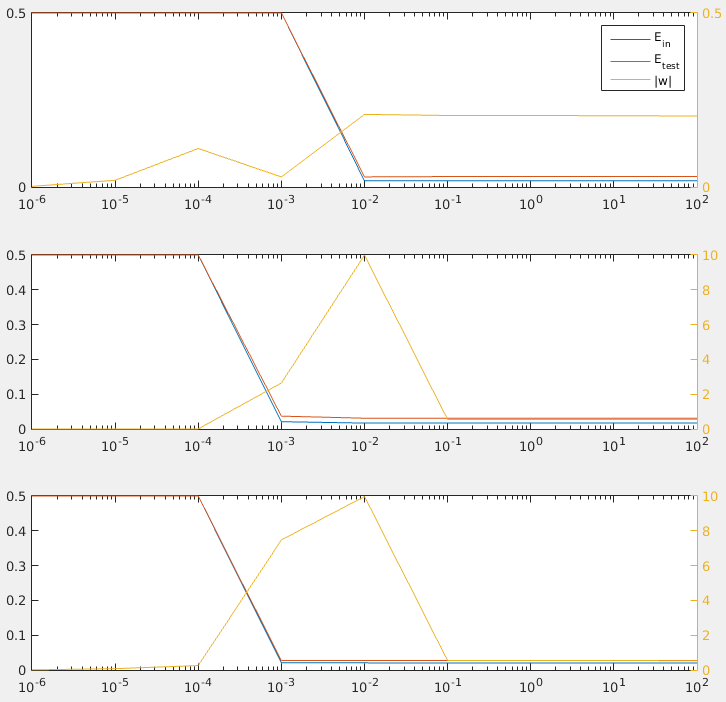
\includegraphics[width=\textwidth]{./01.png}
  \caption{$E_{in}$, $||w||$, and $E_{test}$ as a function of $C$, for the first 250, 500, and 1000 occurences of "1" and "0" in the dataset, the top graph is for 250, then 500 and at the bottom 1000.}
  \label{jegerhomo}
\end{figure}
\noindent We do the same for the digits "0" and "8", this can be seen in Figure \ref{sutminfedepik}.
\begin{figure}[H]
  \centering
  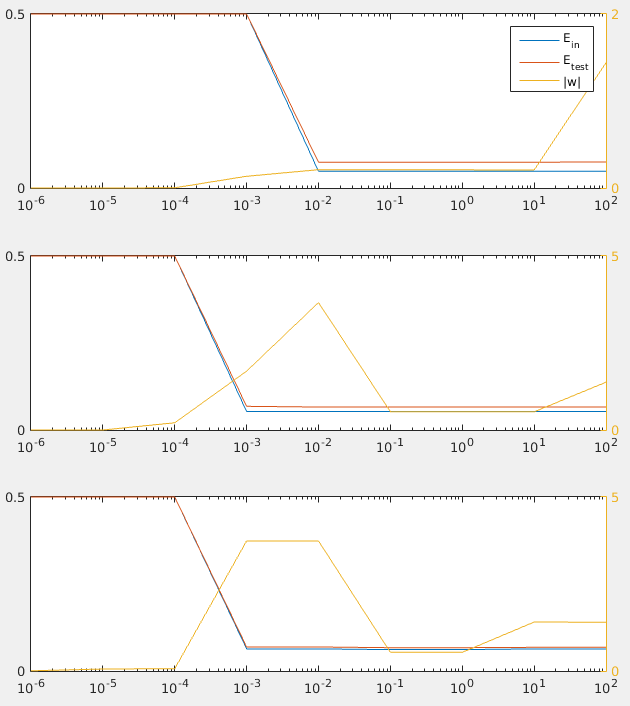
\includegraphics[width=\textwidth]{./08.png}
  \caption{$E_{in}$, $||w||$, and $E_{test}$ as a function of $C$, for the first 250, 500, and 1000 occurences of "8" and "0" in the dataset, the top graph is for 250, then 500 and at the bottom 1000.}
  \label{sutminfedepik}
\end{figure}
\noindent We do the same for the digits "5" and "6", this can be seen in Figure \ref{dueretulideligtmenneske}.
\begin{figure}[H]
  \centering
  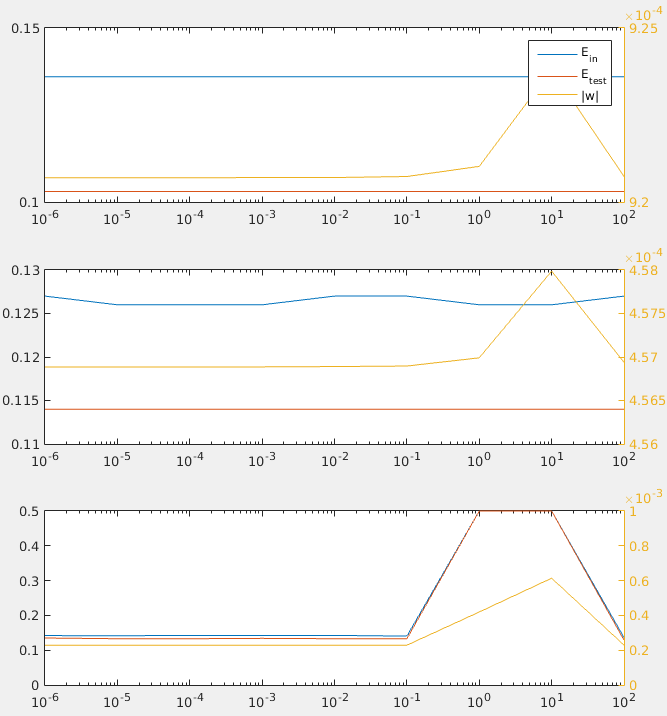
\includegraphics[width=\textwidth]{./56.png}
  \caption{$E_{in}$, $||w||$, and $E_{test}$ as a function of $C$, for the first 250, 500, and 1000 occurences of "5" and "6" in the dataset, the top graph is for 250, then 500 and at the bottom 1000.}
  \label{dueretulideligtmenneske}
\end{figure}



\end{document}